\documentclass[12pt,a4paper,landscape]{article}

\usepackage{pagecolor, afterpage}
\usepackage{eurosym,graphicx,multicol,float}
\usepackage[pdfborder={0 0 0},pdfhighlight=/P]{hyperref}
\usepackage[margin=2cm]{geometry}
\title{\Huge \textbf{The Pop Button}}
\date{}
\author{Kentin and Nil}
\graphicspath{{images/}}

\usepackage[strict]{changepage}

\begin{document}

\definecolor{mycol1}{rgb}{1, 1, 1}
\definecolor{mycol2}{rgb}{1, 1, 1}
\definecolor{mycol3}{rgb}{1, 1, 1}
\definecolor{mycol4}{rgb}{1, 1, 1}

%\definecolor{mycol1}{rgb}{0.95, 0.95, 0.9}
%\definecolor{mycol2}{rgb}{0.95, 0.95, 0.9}
%\definecolor{mycol3}{rgb}{0.95, 0.95, 0.9}
%\definecolor{mycol4}{rgb}{0.95, 0.95, 0.9}

%\definecolor{mycol1}{rgb}{0.7, 0.8, 1}
%\definecolor{mycol2}{rgb}{0.8, 0.9, 0.5}
%\definecolor{mycol3}{rgb}{0.8, 0.6, 0.9}
%\definecolor{mycol4}{rgb}{0.8, 0.4, 0.6}

\pagecolor{mycol1}
\maketitle

\centering{
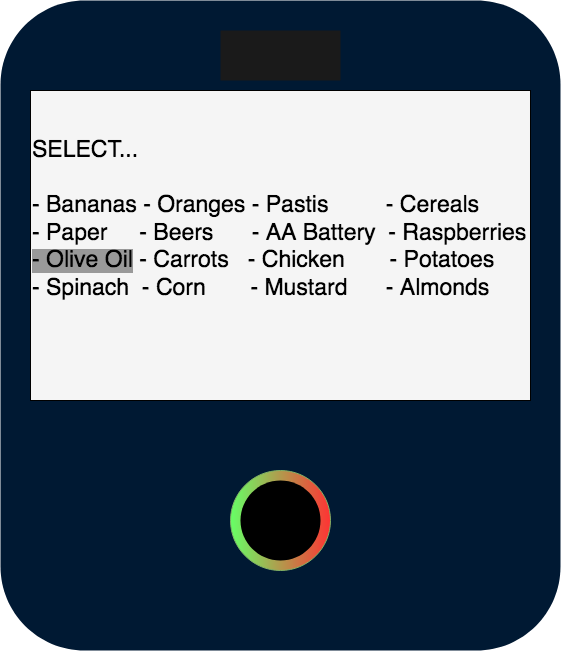
\includegraphics[width=10cm]{pop_button.png}
}
\newpage
\newpagecolor{mycol2}

\section*{\centering Introduction}

	\vspace{4em}

	\begin{adjustwidth}{15em}{15em}
		\centering
	Do you know Sonia?
	
	\vspace{1em}

	Sonia is a young mum, her little baby is sick and she needs to buy some medication.
	So she, as everyone in 19th century, grabs a piece of paper and notes down the medicine along other things as the eggs she needs for Patrick's birthday's cake...
	
	The day after, at the grocery she realizes that she left the list on the fridge and forgot about the medication, once she came back at home the baby was dying and the neighbour had called the police... She is now serving 5 years at Guantanamo for medical negligence.

	\vspace{2em}

	Did you ever experienced something similar ???\\

	Do you want to go in Guantanamo ???\\

	\vspace{3em}
	
	Don't worry we have the solution :
	
	\subsection*{\centering The Pop Button !}
	
	The POP Button is a little device that fits in your cosy place and allows you to keep track of whatever item you need on the cloud in order for you manage it the most efficient way.
	
	If Sonia would have had a POP Button, once she realized she forgot the list on the fridge, she would have been able to connect with her smartphone to our server and find back all the items she entered thanks to her POP friend.
	\end{adjustwidth}

\newpage
\newpagecolor{mycol3}
\section*{Block Diagram}
	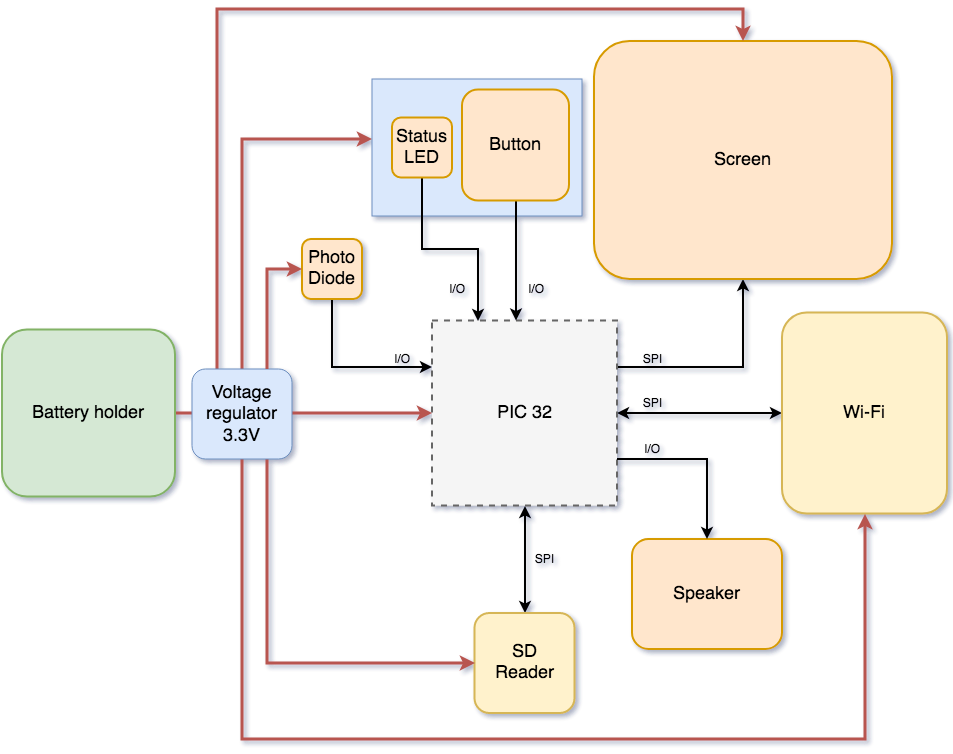
\includegraphics[width=19cm]{block-diagram.png}

\newpage
\newpagecolor{mycol2}
\section*{Manual}
	\begin{multicols}{2}
		\subsection*{First Use / Configuration}
		Before using the POP Button you have to configure the SD Card, connect the SD Card to a computer and use our program to format it.\\
		To use the product for the first time open the rear panel to reveal the battery and SD Card slot. First, put the SD Card in and then put the AA-type batteries. Finally, make sure the switch is in the On position and close the back panel.\\
		Now the screen should light up and you can start to use your product normally. If it doesn't, refer to the troubleshooting section.
		\subsection*{Normal Use}
		Usually, the screen will be turned off and the device will be in sleep mode. The screen should light up when you approach your hand to the device, if it doesn't, press the knob to turn on the screen.

		Once the screen is lit up, you can select the product you want by turning the knob to change the selected item.

		Once you're done, the screen will show you a confirmation and you will hear a sound to confirm the order, also the knob will change it's color accordingly.
		\subsection*{Settings}
		Most advanced settings are edited via the SD Card. But some of them can be edited through the machine.
		To enter settings, long-press the knob. Once you are in the menu, select the desired option and press the button. Now you can adjust the value and push again to validate.
		\subsection*{Knob Color Codes}
			\begin{tabular}{|c|c|p{4.3cm}|}
			\hline
				Off & Sleep & When the button is off it means that the device is in sleep mode\\
				\hline
				Blue & Ready & The device just turned on\\
				\hline
				Orange & Working & The order has been recorded but the device is still sending it to the server\\
				\hline
				Green & Done & The order was processed successfully\\
				\hline
				Red & Error & The device encountered an error\\
				\hline
				Blinking Red & Low Battery & The device is running out of battery. The screen won't turn on until you replace the batteries.\\
				\hline
			\end{tabular}
		\subsection*{Troubleshooting}
		Almost all of the errors can be resolved by following the on-screen instructions. However, here are some other problems that might arise:
		\begin{figure}[H]
			\centering
			\begin{tabular}{|c|p{5cm}|}
				\hline
				Symptom & Solution\\
				\hline
				The device won't turn on & Check that the switch on the back is turned on.\\
				\hline
			\end{tabular}
		\end{figure}
	\end{multicols}

\vspace{2cm}

\newpage
\newpagecolor{mycol1}

\section*{Protocols}
	\begin{multicols}{2}
		\subsection*{UART}
		UART stands for "Universal Asynchronous Receiver Transmitter" it is a little circuit in a micro-controller which transmits and receives serial data.
		As it doesn't use clock it needs to work on a fixed frequency known as the baud rate, the baud rate is explained as bits per second (bps) and both peripherals need to work on the same one in order to communicate.
		When no data is being sent the UART line is in idle state (logic high).
		To send data UART transmits it in packets, this packets are conformed as follows:
		
		\centering{
			\begin{itemize}
				\item 1 Start Bit (To exit the idle state)
				\item 5-9 Data Bits (The actual data)
				\item 1 Optional Parity Bit (Like a checksum)
				\item 1 or 2 Stop Bits (To enter the idle state again)
			\end{itemize}
		}
		
		All of the configuration, like how many data bits, if there will be a parity bit, if there will be 1 or 2 stop bits and the baud rate have to be set beforehand.

		\begin{center}
			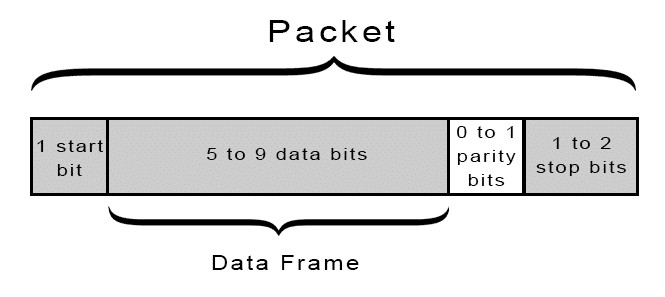
\includegraphics[width=12cm]{UART_packet.png}
		\end{center}

		\vspace{4cm}

		\subsection*{SPI}
		SPI stands for ”Serial Peripheral Interface” it is a synchronous and full-duplex communication protocol, which means that it uses a clock and it can receive and send at the same time
This protocol uses 3 lines to work and then one pin more for each slave to in order to select it:

		\begin{itemize}
			\item SCLK $\Rightarrow$ Serial Clock 
				(SCK, SCL)
			\item MOSI $\Rightarrow$  Master Output, Slave Input
				(SDI, DI, SI)
			\item MISO $\Rightarrow$  Master Input, Slave Output  
				(SDO, SDA, DO, SO)
			\item SS $\Rightarrow$  Slave Select
				(nCS, CS, nSS, STE, CSN)
		\end{itemize}
		So first the master has to select a slave, to do so it lowers the appropiate `SS` line. To send the data they must have agreed in the settings for Clock Polarity and Clock Phase.\\
		There are 4 modes available:

		\vspace{1em}
		\begin{tabular}{|c|c|c|}\hline
			SPI mode & CPOL & CPHA \\\hline
			0        & 0    & 0    \\\hline
			1        & 0    & 1    \\\hline
			2        & 1    & 0    \\\hline
			3        & 1    & 1    \\\hline
		\end{tabular}

		The master then turns on the clock. To send the data, the master uses the `MOSI` line and the slave uses the `MISO`. They send one bit per clock cycle, the exact timing specific is determinated by the Clock Settings. And can be seen in the following graphic. In the clock waveform there are two states the 'send' mode and the 'capture' mode. The data lines (MISO, MOSI) cannot change while the clock is on the capture mode. They can only do it while in the 'send' mode.

		\begin{center}
				\includegraphics[width=12cm]{SPI_timing.png}
		\end{center}

		One thing to have in account is that: As the master is the one that's responsible for keeping the clock signal alive it has to keep sending the clock signal if it won't send data but expects data from the slave.\\

		\vspace{0.5cm}

		Once the comunication with that slave has ended the SS is raised again. And then the slave puts the MISO line in high impedance mode.
	
		\vspace{4cm}

		\subsection*{\texorpdfstring{i$^{2}$C}{}}
		I$^2$C or IIC stands for Inter-Integrated Circuit, it is a protocol which is synchronous, half-duplex, multi-master and multi-slave. It can address between 127 and 1024 devices but is slower than SPI
		Exchange alway take place between one master and one are all slaves\\
		It is possible for devices to pass from master to slave and vice versa.\\
		The connexion is handled by two lines
		\begin{itemize}
			\item SCL $\Rightarrow$ Serial Clock Line bidirectionnal data line\\
			\item SDA $\Rightarrow$ Serial Data Line bidirectionnal synchronisation line
		\end{itemize}
		Those two lines are pull to VDD Voltage with pull-ups resistors.\\
		The maximal number of peripheral is limited by the address size of 7 bit and the capacitance of the bus.
		There is reserved address space by some makers and for the broadcast\\
		SDA levels HIGH or LOW have to be maintained during HIGH leve of the SCL.
		With multiple compnents, due to the fact that default state is HIGH the zero state is dominant and a one state emmited by another componant will be erased
		There is five transmission speeds
		\begin{itemize}
			\item Sm $\Rightarrow$ Standard mode $\leq$ 100 kbit/s
			\item Fm $\Rightarrow$ Fast mode $\leq$ 400 kbit/s
			\item Fm+ $\Rightarrow$ Fast plus mode $\leq$ 1 Mbit/s
			\item Hs-mode $\Rightarrow$ High-speed mode $\leq$ 3.4 Mbit/s
			\item UFm $\Rightarrow$ Ultra-fast mode $\leq$ 5 Mbit/s (one-way communication only)
		\end{itemize}
		There is minimum time for the state to be HIGH or LOW\\
		\vspace{1em}
		\begin{tabular}{|c|c|c|}
			\hline
			Mode & \raisebox{0.2em}{\small t}LOWmin & \raisebox{0.2em}{\small t}LOWmin \\
			\hline
			Standard & 4.7 $\mu$s & 4 $\mu$s \\
			Fast & 1.3 $\mu$s & 0.6 $\mu$s \\
			Fast plus & 0.5 $\mu$s & 0.26 $\mu$s \\
			\hline
		\end{tabular}

		\subsubsection*{Master $\leftrightarrow$ Slave exchange}

		\begin{itemize}
			\item The master is emitting and the slave receives
			\begin{itemize}
				\item emission of the start condition by the master
				\item emission of one more address byte by the master to select the slave with the R/W bit at 0
				\item answer of the slave with a ACK (or NACK)
				\item after each ACK the slave can ask a break
				\item emission of a command byte of the master to the slave
				\item answer of the slave (ACK or NACK)
				\item emission of a restart condition by the master
				\item emission of the address byte or bytes by the master to select the same slave with the R/W bit at 1
			\end{itemize}
			\item The master become receiver and the slave emitter
			\begin{itemize}
				\item emission of a data byte by the slave to the master
				\item answer of the master with an ACK/NACK
				\item emission of more byte depending of the ammount of data the master is asking
				\item for the last byte the master respond with a NACK to stop the dialog
				\item master emit a STOP condition
			\end{itemize}
		\end{itemize}

		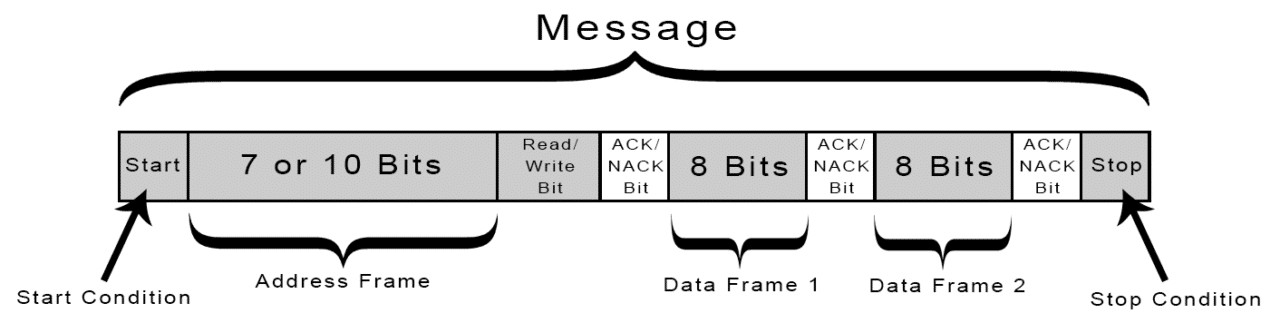
\includegraphics[width=13cm]{I2C_packet.png}

	\end{multicols}

	{\color{blue}In order to start, stop and restart a transmission the master can transgress the codage rule\\}

		\vspace{1em}

			\begin{tabular}{p{7cm}p{7cm}p{7cm}}
				Start condition by passing SDA from HIGH to LOW during SCL is HIGH
				\newline \newline \newline
				\parbox[]{1em}{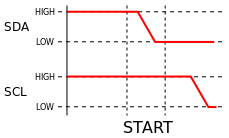
\includegraphics[width=6cm]{START_I2C.png}} &
				Stop condition by passing SDA from LOW to HIGH during SCL is HIGH
				\newline \newline \newline
				\parbox[]{1em}{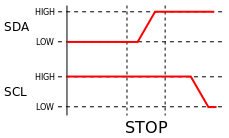
\includegraphics[width=6cm]{STOP_I2C.png}} &
				Restart condition by passing SDA from HIGH to LOW just after SCL past from LOW to HIGH
				\newline \newline
				\parbox[]{1em}{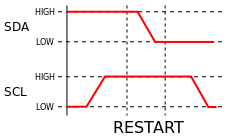
\includegraphics[width=6cm]{RESTART_I2C.png}}\\
			\end{tabular}

\newpage
\newpagecolor{mycol3}

\section*{Specifications}
	
	\vspace{6em}

	\begin{itemize}
		\item eXtreme Low Power PIC32
		\item 256K Flash
		\item 64K SRAM
		\item 2.4GHz Wi-Fi Connection
		\item 320 x 240 pixel TFT LCD screen 2.8"
		\item Endless rotary button
		\item RGB LED
		\item Maximum distance to activate the device of 76.2 mm
		\item 70dB buzzer
		\item 4 x AA Batteries Required
		\item 3 months autonomy
	\end{itemize}

\vspace{2cm}

\newpage
\newpagecolor{mycol2}

\section*{So what do we need ?}
	\begin{multicols}{2}
	\subsection*{A PIC}
		\begin{figure}[H]
		\centering
		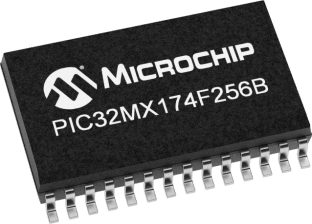
\includegraphics[height=4cm]{images/pic32.png}
		\end{figure}
		The choice of the PIC have been done mostly on the power consumption performance and the availability on farnell as well as the number of SPI ports.

	\subsection*{A Button}
			\begin{figure}[H]
			\centering
			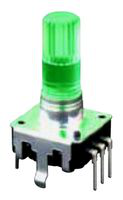
\includegraphics[height=4cm]{images/rotary_encoder.png}
			\end{figure}
			We chose this encoder because it fits exactly our needs: it rotates infinitly either way, it has a push button integrated enabling the ability to choose and select within an instant, further to that it also has an RGB led incorporated !

	\subsection*{A Wifi Module}
			\begin{figure}[H]
			\centering
			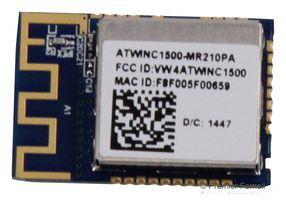
\includegraphics[height=4cm]{images/atwinc1500.png}
			\end{figure}
			In order to communicate with the server we needed a wifi connection that we found in the atwinc1500, this module is compatible with most wifi encryption and has an SPI interface as well as a low-power mode.

	\subsection*{A screen}
			\begin{figure}[H]
			\centering
			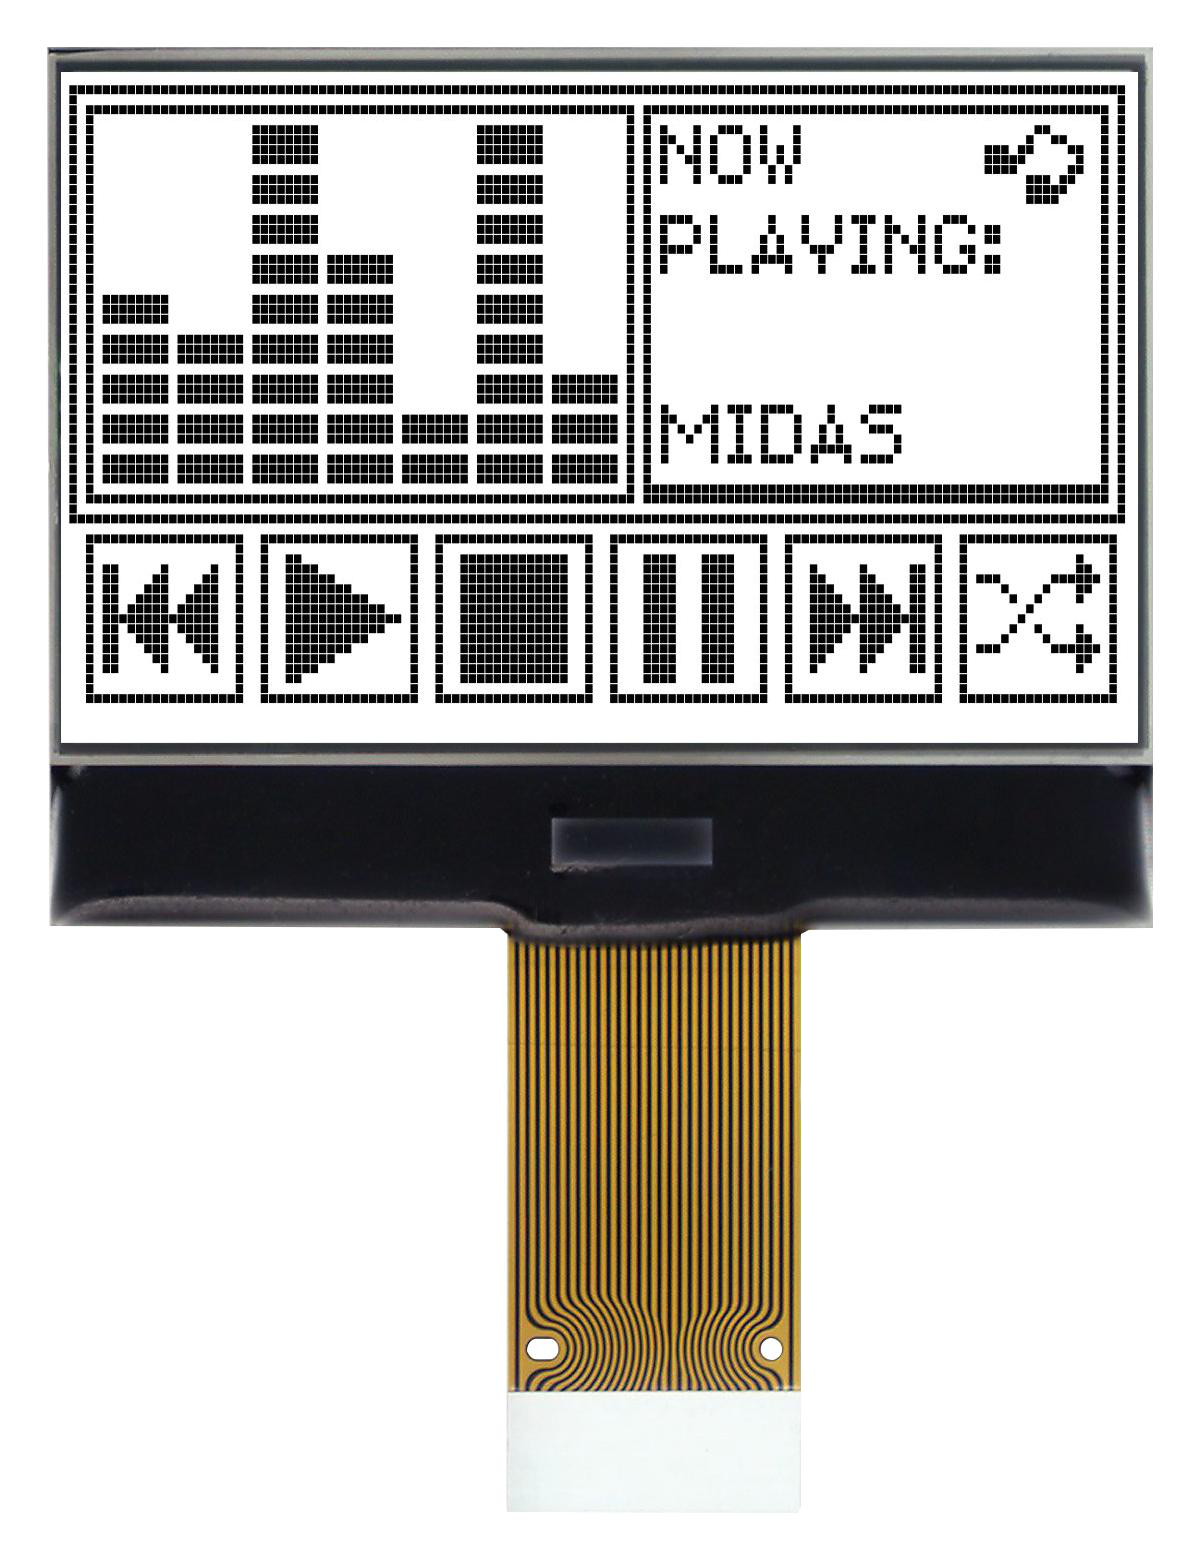
\includegraphics[height=4cm]{images/screen.png}
			\end{figure}
			We chose this screen because it is large enough to contain a good list of words,it has an English and Japanese font set, it is bright so we can see it in different environnements and it is 3.3V powered wich make it easy to interface with all other modules.

	\subsection*{A screen second choice}
			\begin{figure}[H]
			\centering
			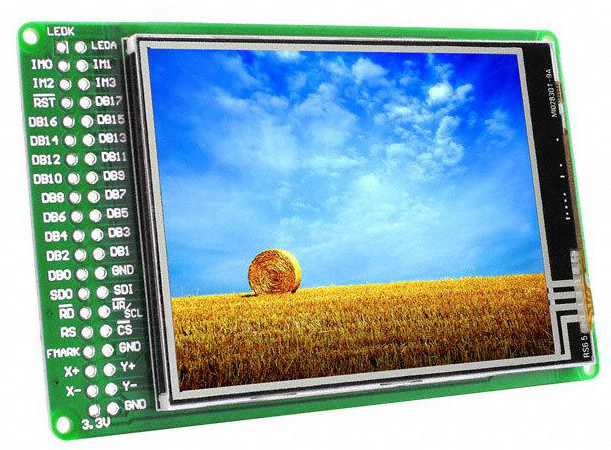
\includegraphics[height=4cm]{images/screen2.png}
			\end{figure}
			This screen has easy connector compare with the other one and is widely used so it can be easy to find documentation on internet, it is 3.3V unlike other black and white screen

	\subsection*{Memory Socket}
			\begin{figure}[H]
			\centering
			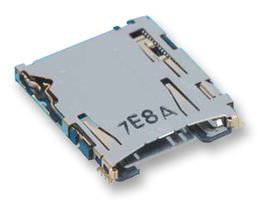
\includegraphics[height=4cm]{images/memory_socket.png}
			\end{figure}
			As a compusilve buyer you will need a lot of products in your list, that's why we chose to add a memory extension.

			\vspace{4cm}

	\subsection*{Photo-Diode}
			\begin{figure}[H]
			\centering
			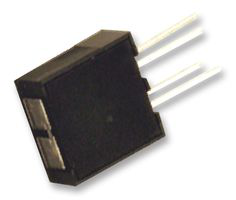
\includegraphics[height=4cm]{images/photo-diode.png}
			\end{figure}
			Thanks to the half-god Gregory Le Grand we will use a photo-diode to interact with the device, we chose this one because it can detect a distance of 7.4cm instead of 2.5 for most devices

	\subsection*{Piezo}
			\begin{figure}[H]
			\centering
			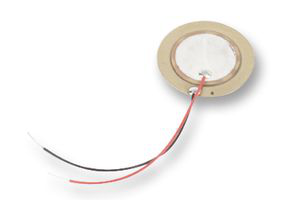
\includegraphics[height=4cm]{images/piezo.png}
			\end{figure}
			Because everyone loves music, we necessarily wanted a good audio interface that satisfies this requirement.

	\subsection*{Switch}
			\begin{figure}[H]
			\centering
			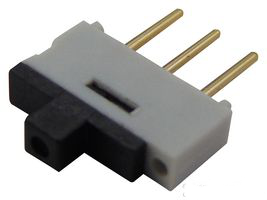
\includegraphics[height=4cm]{images/switch.png}
			\end{figure}
			This basic switch will be the one to turn all the lights off, in order to store the product we want a way to switch it completly off keeping the batteries inside

			\vspace{4cm}
	\subsection*{Battery Holder}
			\begin{figure}[H]
			\centering
			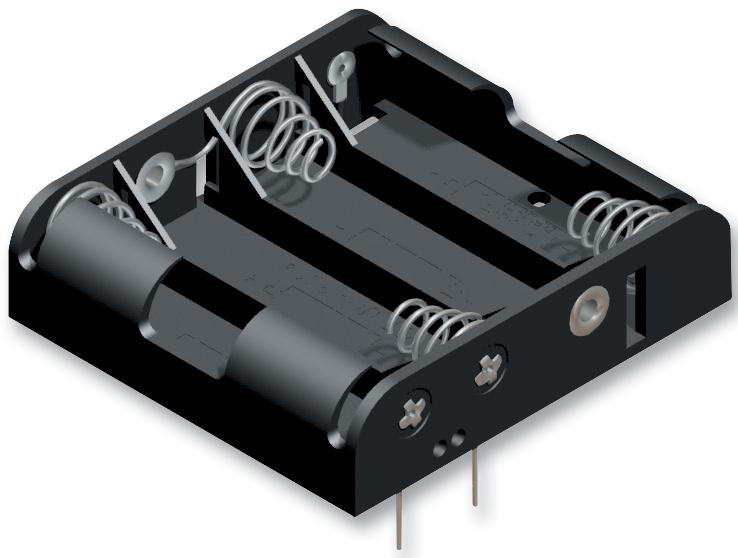
\includegraphics[height=4cm]{images/battery_holder.png} 
			\end{figure}
			Because it wont hold itself...\\
			We chose this one because it widely used, well appreciated and we needed enough mAh to be able to use the device during several months 

			we have 4 AA batteries holding each one 2850mAh 

			4 * 2850 = 11400 

			Our device consumes at most 500mA in case everything is working at the same time\\

			so 11400/500 = 22.8 hours the hard way\\

			considering that we use the device 15 minutes a day we use it 7h45 by month 

			 22 / 7.75 = 2,84 months 

			In this conditions we can use the device during three months without changing the batteries which is acceptable.
	\end{multicols}

	\vspace{3cm}

\newpage
\newpagecolor{mycol4}
\section*{References and links}

	\vspace{5em}

			\center{
				We need to be more precise on the consumption, the voltage regulator might not use more than the pic or the screen...\\
				I didn't find a good approximation of the pic consumption\\
				So we have to know on witch frequency the pic will work with the ATWINC and without (idle mode and sleep mode)

				\vspace{5em}

				\begin{tabular}{|c|c|c|c|c|c|}\hline
					component & reference & price(\euro) & consumption & Frequency & Datasheets \\
					\hline
					
					SoC &
					\href{http://fr.farnell.com/microchip/pic32mx174f256b-i-so/mcu-32-bits-pic32mx-72mhz-soic/dp/2775021?st=PIC32MX174F256B}
					{PIC32MX174F256B-I/SO} & 3.48 & $\sim$ 200mA  @ 3.3V = 660mW &
					72Mhz &
					\href{http://www.farnell.com/datasheets/2244305.pdf}{
\includegraphics[height=1em]{pdf.png}}
					\href{http://ww1.microchip.com/downloads/en/DeviceDoc/80000739A.pdf}{
\includegraphics[height=1em]{pdf.png}}\\
					
					Wi-Fi &
					\href{http://fr.farnell.com/microchip/atwinc1500-mr210pb1952/mod-iot-smartconnect-2-472ghz/dp/2759346?st=atwin}
					{ATWINC1500}  & 6.61 & 70mA / 172mA @ 3.3V = 564mW &
					26Mhz &
					\href{http://ww1.microchip.com/downloads/en/DeviceDoc/Atmel-42420-WINC1500-Software-Design-Guide_UserGuide.pdf}{
\includegraphics[height=1em]{pdf.png}}
					\href{http://www.farnell.com/datasheets/2286658.pdf}{
\includegraphics[height=1em]{pdf.png}}\\

					Screen &
					\href{http://fr.farnell.com/midas/mcot128064h1v-wm/afficheur-graphique-oled-tab-128x64/dp/2817924?st=oled}
					{MCOT128064H1V-WM} & 17.56 & &
					- &
					\href{http://www.farnell.com/datasheets/2549026.pdf}{
\includegraphics[height=1em]{pdf.png}}\\
					
					Screen Power Supply &
					\href{http://fr.farnell.com/texas-instruments/tlv61046adbvt/convert-dc-dc-boost-1mhz-sot-23/dp/2766885?ost=TLV61046ADBVT}
					{TLV61046ADBVT} & 0.96 & &
					- &
					\href{http://www.ti.com/lit/ds/slvsd82a/slvsd82a.pdf}{
\includegraphics[height=1em]{pdf.png}}\\
					
					Screen Connector &
					\href{http://fr.farnell.com/hirose-hrs/fh41-31s-0-5sh-05/conn-ffc-embase-31voies-1rangee/dp/2427829}
					{FH41-31S-0.5SH(05)} & 1.91 & &
					- &
					\href{http://www.farnell.com/datasheets/2169332.pdf}{
\includegraphics[height=1em]{pdf.png}}\\
					
					Screen Connector Breakboard &
					\href{http://uk.farnell.com/roth-elektronik/re918/fpc-ffc-adaptor-fibreglass-1-5mm/dp/2474691?st=adaptor}
					{RE918} & 1.90 & &
					- &
					\href{http://www.farnell.com/datasheets/2169332.pdf}{
\includegraphics[height=1em]{pdf.png}}\\
					
					Rotary Encoder &
					\href{http://fr.farnell.com/alps/ec11e15244c0/encodeur-vert-30-crans-15-impul/dp/1520806?st=boutton}
					{EC11E15244C0} & 3.32 & 10mA @ 5V = 50mW & 
					- &
					\href{http://www.farnell.com/datasheets/5205.pdf}{
\includegraphics[height=1em]{pdf.png}}\\
					
					Photo-Diode &
					\href{http://fr.farnell.com/optek-technology/opb732/capteur-reflectif-pcb/dp/1226877}
					{OPB732} & 3.2 & 50mA @ 3.3V = 165mW &
					- &
					\href{http://www.farnell.com/datasheets/2331536.pdf}{
\includegraphics[height=1em]{pdf.png}}
					\href{http://www.mouser.com/ds/2/414/OP265-266-45966.pdf}{
\includegraphics[height=1em]{pdf.png}}\\
					    
					Voltage Regulator for Photo-Diode &
					\href{http://fr.farnell.com/texas-instruments/tlv73318pdbvt/regulateur-ldo-0-3a-1-8v-sot-23/dp/2455141}
					{TLV73318PDBVT} & 0,0949 & &
					- &
					\href{http://www.ti.com/lit/ds/symlink/tlv733p.pdf}{
\includegraphics[height=1em]{pdf.png}}\\

					Buzzer &
					\href{http://fr.farnell.com/pro-signal/abt-460-rc/buzzer-electro-m-canique-2v-4v/dp/2783902}
					{ABT-460-RC} & 1.55 & &
					- & \href{http://www.farnell.com/datasheets/2362849.pdf}{
\includegraphics[height=1em]{pdf.png}}\\
					    
					Voltage Regulator 3.3V &
					\href{http://fr.farnell.com/texas-instruments/tps561208ddct/dc-dc-conv-sync-buck-580khz-sot/dp/2766883}
					{TPS561208DDCT} &  0.737 & &
					- &
					\href{http://www.ti.com/lit/ds/symlink/tps561201.pdf}{
\includegraphics[height=1em]{pdf.png}}\\
					    
					Micro SD socket &
					\href{http://fr.farnell.com/hirose-hrs/dm3at-sf-pejm5-40/connecteur-micro-sd-push-push/dp/1764374}
					{DM3AT-SF-PEJM5(40)} & 2.64 & &
					- &
					\href{http://www.farnell.com/datasheets/1697167.pdf}{
\includegraphics[height=1em]{pdf.png}}\\
					    
					Battery Holder &
					\href{http://fr.farnell.com/keystone/2477/battery-holder-pcb/dp/1650684}
					{2477} & 1.41 & &
					- &
					\href{http://www.farnell.com/datasheets/1703957.pdf}{
\includegraphics[height=1em]{pdf.png}}\\
					    
					Switch &
					\href{http://fr.farnell.com/c-k-components/l102011ms02q/commutateur-lateral-spdt/dp/2435160}
					{L102011MS02Q} & 1.31 & &
					- &
					\href{http://www.farnell.com/datasheets/1839859.pdf}{
\includegraphics[height=1em]{pdf.png}}\\

					Crystal &
					\href{http://fr.farnell.com/txc/9c-8-000meej-t/xtal-8-000mhz-18pf-smd-hc-49s/dp/1842347}
					{9C-8.0000MEEJ-T} & 0.604 & &
					- &
					\href{http://www.farnell.com/datasheets/1497895.pdf}{
\includegraphics[height=1em]{pdf.png}}\\
					    
					Shift Register &
					\href{http://fr.farnell.com/nexperia/74hc595d/circuit-logique-74hc-cms/dp/1201269}
					{74HC595D} & 0.282 & &
					- &
					\href{http://www.farnell.com/datasheets/2038613.pdf}{
\includegraphics[height=1em]{pdf.png}}\\
					    
					LED &
					\href{http://fr.farnell.com/kingbright/l-154a4sureqbfzgew/led-multicol-rgb-5mm-x-brillant/dp/2290375}
					{L-154A4SUREQBFZGEW} & 0.965 & &
					- &
					\href{http://www.farnell.com/datasheets/2046653.pdf}{
\includegraphics[height=1em]{pdf.png}}\\
					    
					Transistor &
					\href{http://fr.farnell.com/nexperia/2n7002pw/mosfet-canal-n-60v-0-3a-sot323/dp/1829184}
					{2N7002PW} & 0.195 & &
					- &
					\href{http://www.farnell.com/datasheets/1760698.pdf}{
\includegraphics[height=1em]{pdf.png}}\\
					    
					\hline
					total & & & & &\\
					\hline
				\end{tabular}
			}
\end{document}
